\documentclass[journal]{IEEEtran}

\usepackage[T1]{fontenc}
\usepackage{newtxtext,newtxmath}
\usepackage{graphicx}
\usepackage{booktabs}
\usepackage{amsmath}
\usepackage{url}
\usepackage[hidelinks]{hyperref}

\newcommand{\rupee}{INR\,}

\begin{document}

\title{Varuna FloodTwin: An Open Urban Flood Digital Twin\\ Built from Free Satellite Data, and an Honest\\ Measurement of What It Can Predict}

\author{Ansh~Vivek%
\thanks{The author is an independent researcher (e-mail: anshvivek2003@gmail.com).}%
\thanks{Code, all per-area data bundles and the live system are public. Repository:
\url{https://github.com/Maverick-Ansh/project-varuna}. Dashboard:
\url{https://project-varuna-iota.vercel.app}. API:
\url{https://anshvivek-varuna-floodtwin.hf.space}.}}

\markboth{Preprint}{Vivek: Varuna FloodTwin}

\maketitle

\begin{abstract}
Cities in India flood every monsoon, and most of them have no calibrated flood model to plan with.
We present Varuna FloodTwin, an open pipeline that builds a working flood model of any place on
Earth from free satellite data, runs it fast enough to answer questions live in a web page, and
serves it for 16 city areas in India. Every stage runs on free computing tiers. Our main claim is
not that the model is accurate. It is that we measured what such accuracy numbers are worth, and
the answer changes how they should be read. On 150 Sentinel-1 radar scenes across 15 city areas, a
baseline with no physics and no rainfall, which simply predicts the cells that were wet in most
other storms, scores a Critical Success Index (CSI, the standard flood overlap score) of 0.29 to
0.67. That is higher than any physics-model CSI we can find published for this task, including our
own. In all 15 areas it is also higher than the agreement between two radar passes of the same
city, which is a ceiling on what any model can be asked to match. Our physics twin scores 0.054,
and a learned model reading the same terrain rasters scores 0.288, which ties the no-physics
baseline to three decimal places. The learned model's real value is therefore not accuracy but
portability, because it still runs on a city with no radar archive, where the baseline cannot be
computed at all. Holding out one entire region at a time it scores 0.147, and a threshold
correction that never looks at a test label raises this to 0.175. That correction helps most
exactly where the model is weakest, lifting held-out coastal Mumbai from 0.061 to 0.106. Rainfall
from free reanalysis contributes nothing at any grouping level, shown four independent ways.
Neither model size, from 2.0 to 70.6 million parameters, nor grid resolution, from 60\,m to 30\,m,
moves the result. We then show that planning survives this location uncertainty, because the value
of every intervention is measured by re-simulation rather than assumed. A dense storm drain network
routed on the real street graph cuts simulated street flooding by 80.9\,\% in Patna at a lower cost
per cubic metre removed than sparse canals, and a metered recharge planner sends 6.3 to 16.5\,\% of
storm runoff into depleted aquifers in six Karnataka towns against 0.7 to 3.3\,\% on flood plains.
An inferred drainage field puts Mumbai's whole-city drainage ceiling near 5.4 million cubic metres
per storm, just above the 4.7 million cubic metres per day the municipal corporation measured
pumping in August 2025, which is our first external anchor. Finally, a graph neural network over
the street graph amortizes the raster pipeline into a 4.1\,ms per-street risk query against
260\,ms, transfers to an unseen city at AUC 0.72 to 0.85, and produces evacuation routes recovering
64.6\,\% of an oracle's floodwater avoidance at 57\,\% of its detour.
\end{abstract}

\begin{IEEEkeywords}
Urban flooding, digital twin, Sentinel-1, synthetic aperture radar, flood validation, graph neural
networks, managed aquifer recharge, open data.
\end{IEEEkeywords}

\section{Introduction}
\IEEEPARstart{P}{luvial} flooding, which means flooding caused by rain falling on the city itself
rather than by a river bursting its banks, is one of the most frequent climate impacts in South
Asian cities. The planning reality in most Indian municipalities is a drainage map older than the
city that grew around it, no calibrated hydraulic model, and no budget to buy one.

A tool that could change decisions in that setting has to meet three conditions. It must be
buildable from free and global data for any area, because nobody is going to survey the city for
us. It must be cheap enough to run interactively, because planning is a conversation and not a
batch job. And it must be honest about what it can and cannot claim, because a confident wrong
answer about which street floods is worse than no answer at all.

This paper describes such a system, and it also argues for a particular way of reporting its skill.
Fig.~\ref{fig:teaser} is what a planner actually sees. It is a live map of Patna at a chosen
rainfall. Blue shading is predicted water depth, arrows point the way water is flowing, orange
circles are drain inlets the system placed, purple lines are the storm drain network it designed,
and the dark labels name real roads with a depth a person can picture.

\begin{figure*}[!t]
\centering
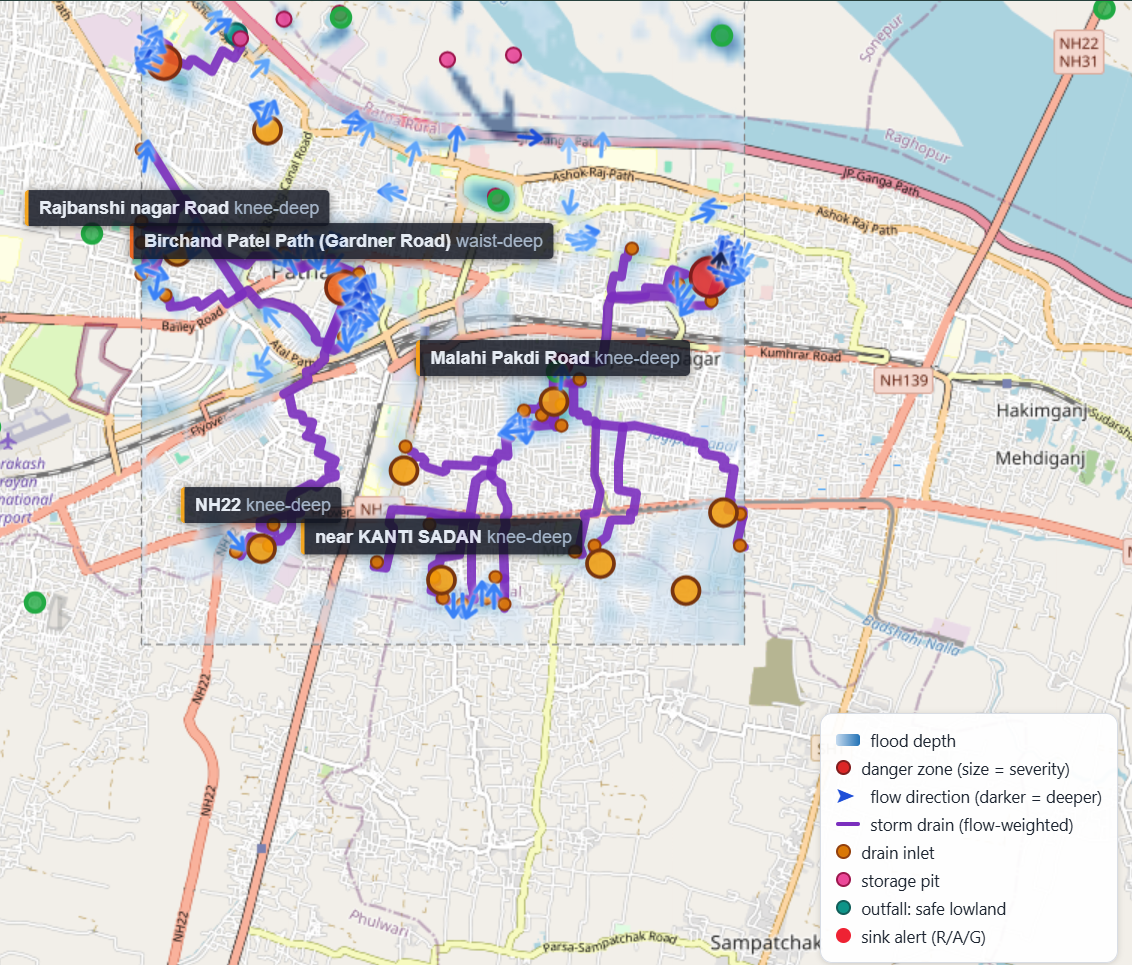
\includegraphics[width=0.93\textwidth]{figures/live_patna_city.png}
\caption{The live system for Patna at a 100\,mm design storm. Blue shading is predicted water depth
and the arrows show flow direction, with darker arrows meaning deeper water. Purple lines are the
storm drain network the planner designed on the real street graph, and the line gets wider as more
water accumulates in that trunk. Orange circles are drain inlets, pink circles are storage pits,
and green circles are outfalls placed on safe low ground rather than on the river. Red circles are
danger zones sized by severity. The dark labels name real streets and give the depth in words,
because ``waist-deep'' is a decision and ``0.94\,m'' is only a measurement. Everything here is
computed from free satellite data and served from a free hosting tier.}
\label{fig:teaser}
\end{figure*}

Our contributions are the following.

\begin{enumerate}
\item \textbf{A reproducible pipeline from satellite to dashboard on free infrastructure.} A
      differentiable two-dimensional flood model \cite{bates2010} is built per city from FABDEM
      \cite{hawker2022fabdem}, ESA WorldCover \cite{zanaga2021worldcover} and JRC surface water
      \cite{pekel2016}. A U-Net emulator \cite{ronneberger2015} answers what-if questions in
      milliseconds. A public dashboard serves rainfall sliders, planners, exposure views and a
      grounded text brief. It is deployed for 16 city areas.
\item \textbf{A measurement of what a flood CSI is actually worth}, using trivial baselines that
      cost nothing to compute and that we think should accompany every CSI reported in this
      literature.
\item \textbf{Three corrections against our own earlier published claims}, each forced by an
      experiment we ran ourselves, and each reported with the number that forced it.
\item \textbf{A transfer result measured the hard way}, holding out an entire region rather than one
      tile, with a control that rules out the obvious alternative explanation.
\item \textbf{A coverage result for coastal cities}, which turns a suspected hard limit into a
      data-collection instruction.
\item \textbf{A threshold correction that costs nothing} and helps most where the model is worst.
\item \textbf{Planning surfaces whose value is measured by re-simulation}, covering storm drains,
      distributed storage and aquifer recharge, with an external anchor against real municipal
      pumping records.
\item \textbf{A learned street-level risk model} that amortizes the physics, transfers between
      cities without retraining, and routes people around water.
\item \textbf{A reproducibility hazard} in which a fixed random seed made a training failure
      perfectly repeatable, together with the guard that fixes it.
\end{enumerate}

We have tried to write this paper in plain language. Where a technical term is unavoidable, it is
explained the first time it appears.

\section{Related Work}
\textbf{Flood physics.} Our numerical core is the local inertial shallow water scheme of Bates
\emph{et al.} \cite{bates2010}, the reduced-complexity formulation that made metre-scale
two-dimensional urban flood modelling tractable. Its operational descendant is LISFLOOD-FP
\cite{shaw2021lisflood}. Our contribution is not the scheme. It is a re-implementation in PyTorch
so that every simulation is differentiable from end to end, which means we can take the gradient of
the flood with respect to the model's own physical parameters. Recent work moves the same way.
Inunda \cite{li2026inunda} is a near-concurrent GPU-native differentiable solver with essentially
the same core, and universal shallow water equations with differentiable programming
\cite{liu2025uswe} learn a flow-resistance closure inside the full equations. Neither ships an
emulator, a hosted twin or a planning stack, and we do not claim to predate either.

\textbf{Flood digital twins and emulators.} CLDNet \cite{cldnet2026} and FlowsDT \cite{flowsdt2026}
build AI-driven twins for metropolitan flooding. Google's Flood Hub work \cite{nearing2024}
predicts extreme floods in ungauged river basins at global scale, which is the river-flood
counterpart of what we do for rain-driven city flooding.

\textbf{Graph neural networks for flooding.} SWE-GNN \cite{bentivoglio2023swegnn} and its
multi-scale successor \cite{bentivoglio2025mswegnn} put hydraulics into message passing on a mesh.
FloodGNN-GRU \cite{kazadi2024gru} and hydraulics-informed message passing \cite{kazadi2024icml} do
the same for spatio-temporal prediction, and HydroGAT \cite{hydrogat2025} adds graph attention. Our
graph is different in kind. It is the road network itself, so what gets predicted is the flooding
of a named street rather than of a mesh cell, and the training labels are generated by our own twin
rather than by a commercial solver.

\textbf{Validation and elevation uncertainty.} Wing \emph{et al.} \cite{wing2017} set the standard
for validating a continental flood model against observations. Marsh \emph{et al.} \cite{marsh2024}
measure the vertical accuracy of free global elevation models in flood-prone terrain, which is the
error budget driving our own uncertainty analysis in Section~\ref{sec:dem}. Assump\c{c}\~ao
\emph{et al.} \cite{assumpcao2018} and Mazzoleni \emph{et al.} \cite{mazzoleni2017} study whether
citizen observations can improve flood models, which is the question our participatory layer is
built to ask.

\textbf{Drainage design and recharge.} Hesarkazzazi \emph{et al.} \cite{hesarkazzazi2022} generate
optimal centralized and decentralized drainage layouts by graph-theoretic optimisation. On the
water-supply side, managed aquifer recharge as a joint answer to urban floods and groundwater
depletion is studied in \cite{mar2026}, and the Underground Taming of Floods for Irrigation concept
\cite{pavelic2015utfi} is its best-known field implementation in the Ganges basin. Our recharge
planner differs by metering the water it claims to bank through a re-simulated physical model
instead of assuming an infiltration rate.

\textbf{What is missing from this literature.} We could not find a paper in it that reports its CSI
beside a trivial baseline computed on the same scenes. Section~\ref{sec:worth} argues that this
single omission makes most reported flood CSI values impossible to interpret, including the ones we
published ourselves.

%% ---- body sections ----
\section{The System}
\label{sec:system}

\subsection{Build layer, run once per city on a free GPU}
For any area of interest, Google Earth Engine exports four free global datasets. FABDEM
\cite{hawker2022fabdem} gives ground elevation at 30\,m with forests and buildings stripped out, so
that the surface is what water actually runs over. ESA WorldCover \cite{zanaga2021worldcover} gives
land cover at 10\,m, which tells us whether a cell is concrete, soil or vegetation. JRC surface
water \cite{pekel2016} tells us which cells are permanently wet, so that a lake is not mistaken for
a flood. Sentinel-1 radar scenes \cite{torres2012} give observed water on real storm dates, and
radar is used because it sees through cloud, which matters when the thing being observed is a
monsoon.

The model domain is a square grid at 60\,m. Patna-family and Bengaluru bundles use $128^2$ cells,
which is a window about 7.7\,km across, and each Mumbai tile uses $256^2$ cells, about 15.4\,km.
The Mumbai tiles share exact latitude and longitude edges, so adding them up never double-counts
any ground. Those tiles are independent models with closed boundaries, which means water does not
flow from one tile into its neighbour and tides are not simulated. The dashboard says so on the
page.

The solver is the local inertial shallow water scheme of Bates \emph{et al.} \cite{bates2010},
written in PyTorch. Writing it in PyTorch is the point. Every step is differentiable, so we can ask
what change in a physical parameter would have changed the flood, and answer it with a gradient
rather than by trying values one at a time. Land cover classes map to Manning roughness, which is a
number describing how much a surface slows water down, and to infiltration, which is how fast water
soaks into the ground. Rainfall forcing comes from Open-Meteo reanalysis and forecast
\cite{openmeteo}.

\subsection{Metered infiltration, and a physics correction that made our floods worse}
An earlier version let every pervious cell soak up water at a constant rate for as long as the storm
lasted, which is wrong. Real soil fills up. Version~3 meters infiltration against a finite soil
storage capacity and caps the rate at the saturated hydraulic conductivity of the soil, which is
the fastest water can physically move through it. This change makes our predicted flooding
\emph{worse}, by design, and we committed the before and after comparison so the change is
auditable. At Patna and 100\,mm of rain, water that soaks in falls from 465\,449 to
391\,525\,m$^3$, ponded water rises by 1.4\,\%, and predicted flooded area goes from 20.63 to
20.78\,km$^2$. Soil fills to only 2.7\,\% of its capacity in that storm, which is the useful part
of the result. It says the earlier model was not merely mis-parameterised. It was letting a nearly
empty sponge absorb water forever.

\subsection{A millisecond emulator, and a reproducibility hazard}
A U-Net \cite{ronneberger2015} is trained to imitate the solver so the dashboard can answer what-if
questions instantly. Wet cells carry twenty times the weight in the loss, because flooding is rare
in space and a plain average error is minimised by predicting no flood anywhere. Validation error
across the bundles is 5 to 21\,cm and the dose-response is monotone, meaning more rain always
produces more water.

Building this exposed a failure worth reporting. Our dataset generator seeds the global random
number generator so that storm sampling is reproducible. That also makes the network's starting
weights bit-identical on every rebuild. On the Mumbai Island-City tile, where much of the window is
harbour, that particular starting point collapses deterministically. Within one epoch the optimizer
pushes the softplus output head so far negative that its gradient vanishes, and the emulator is
stuck predicting zero water everywhere. The validation error looks plausible at 16.3\,cm, which is
exactly the root mean square of the targets, and it stays frozen to the last digit for 40 epochs.
A frozen metric is the tell, because it means the gradients are exactly zero.

The important part is that rebuilding cannot fix this. We measured three bit-identical collapses
before diagnosing it. A fixed seed makes failures reproducible too. The shipped trainer now detects
a collapsed validation prediction, meaning no cell above the wetness threshold despite wet targets,
and retrains from an explicit alternate seed. The first alternate seed turned the worst tile into
the best-fitting emulator in the system, at 5.0\,cm validation error. We flag the pattern because
build pipelines that reseed globally for data reproducibility are common, and a frozen validation
metric is an easy and general warning sign.

\subsection{Serve layer, on free CPU hosting}
A FastAPI backend serves the committed per-city bundles, including cached OpenStreetMap road graphs
\cite{osm} and exposure counts, so the deployed service needs no external API access at run time.
It re-runs interventions live in seconds. A React and Leaflet front end exposes rainfall what-ifs,
ward alerts, drainage, storage and excavation planners, building and road level exposure, validation
panels, and a text brief grounded in the bundle's own numbers. A night lights layer
\cite{roman2018} overlays satellite-observed power outages. Everything from build to serve fits
inside free tiers, and a new city window takes roughly 15 to 25 minutes to build on a free T4 GPU,
including every artifact the server needs.

The system is deployed for 16 areas. These are Patna and two sub-windows, Bengaluru, six Mumbai
tiles, and six towns in Karnataka. A seventeenth area, Chennai, exists as a data bundle used for
the coastal experiment of Section~\ref{sec:coastal} but is not served, which is why the count of
deployed areas and the count of areas with radar ground truth are different numbers in this paper.

\section{What a Flood CSI Is Actually Worth}
\label{sec:worth}

The most useful thing we can report is not a model score. It is the range a flood score can occupy
on this task \emph{before any model exists}.

\subsection{The score, and the three baselines}
The Critical Success Index is the standard overlap measure in flood mapping. Take the cells the
model says are wet and the cells the radar says are wet. CSI is the number of cells both agree on,
divided by the number of cells either one calls wet. It runs from 0 to 1. Three baselines cost
nothing and bracket it.

\emph{All-wet} predicts every cell is flooded. Its CSI is exactly the observed wet fraction, earned
with zero knowledge. \emph{Random} scatters the correct number of wet cells uniformly at random.
\emph{Climatology} predicts the cells that were wet in most \emph{other} storms of that same area.
It uses no rainfall, no physics and no elevation, and it has one threshold which we fix at 0.5 for
every area rather than tuning it per area, so it is not fitted to the scenes it is scored on. We
also compute a fourth quantity, \emph{SAR versus SAR}, which scores every radar date of an area
against every other radar date of the same area. That is not a baseline. It is an empirical ceiling,
because it measures how much two radar passes of the same city agree with each other.

\begin{table*}[!t]
\centering
\caption{What a CSI is worth on Sentinel-1 flood extent, per area, with no model at all. 150 radar
scenes across 15 areas, of which 149 are scored. Climatology predicts the cells wet in most
\emph{other} storms of that area, with one threshold fixed at 0.5 everywhere. SAR versus SAR scores
every date against every other date of the same area, which is an agreement ceiling between two
radar passes of the same city. Every value is regenerated by \texttt{csi\_net/build\_trivial.py}.}
\label{tab:trivial}
\begin{tabular}{lccccc}
\toprule
area & storms & all-wet & random & climatology & SAR vs SAR \\
\midrule
Patna             &  7 & 0.054 & 0.028 & \textbf{0.286} & 0.214 \\
\midrule
Bengaluru         & 10 & 0.022 & 0.011 & \textbf{0.577} & 0.502 \\
\midrule
Mumbai-South      & 10 & 0.017 & 0.008 & \textbf{0.553} & 0.464 \\
Mumbai-West       & 10 & 0.019 & 0.010 & \textbf{0.464} & 0.387 \\
Mumbai-East       & 10 & 0.020 & 0.010 & \textbf{0.598} & 0.511 \\
Mumbai-North      & 10 & 0.024 & 0.012 & \textbf{0.543} & 0.459 \\
Mumbai-Northeast  & 11 & 0.013 & 0.007 & \textbf{0.391} & 0.271 \\
Mumbai-Harbour    & 11 & 0.021 & 0.010 & \textbf{0.572} & 0.462 \\
\midrule
Chennai           & 10 & 0.021 & 0.011 & \textbf{0.500} & 0.383 \\
\midrule
Doddaballapura    & 10 & 0.014 & 0.007 & \textbf{0.674} & 0.568 \\
Ramanagara        & 10 & 0.009 & 0.004 & \textbf{0.668} & 0.586 \\
Chitradurga       & 10 & 0.019 & 0.010 & \textbf{0.671} & 0.593 \\
Chamarajanagara   & 10 & 0.006 & 0.003 & \textbf{0.522} & 0.464 \\
Kolar             & 10 & 0.030 & 0.015 & \textbf{0.553} & 0.458 \\
Chikkaballapur    & 10 & 0.045 & 0.023 & \textbf{0.604} & 0.523 \\
\midrule
mean              & 149 & 0.022 & 0.011 & \textbf{0.545} & 0.456 \\
\bottomrule
\end{tabular}
\end{table*}

\subsection{The result}
Table~\ref{tab:trivial} is the answer. A climatology with one fixed threshold and no other
parameter scores 0.29 to 0.67, with a mean of 0.545. That is higher than any CSI we are aware of
being reported for a physics-based urban flood model on Sentinel-1, including our own.

It is also higher, \emph{in all fifteen areas}, than the agreement between two Sentinel-1 passes of
that same city. Averaging many passes is more self-consistent than any two of them, which is a
property of the target and not of a model. This caps what any model can honestly be asked to do
here.

The reason the level is so high is that the Sentinel-1 target is dominated by water that has
nothing to do with the storm and that the JRC permanent-water mask does not remove. Tidal flat,
mangrove, seasonal pond and paddy field are all wet on most dates. CSI on this task has therefore
mostly been measuring \emph{can you find standing water}, which our twin never attempted, because
the twin predicts only the water the storm adds.

The signature confirms this reading. On Mumbai-Northeast's one genuine flood, 2026-07-08, with
2\,937 wet cells against a baseline near 450, the climatology scores its \emph{worst} value of
0.075. It wins the quiet dates and loses the flood.

\subsection{What we recommend}
CSI in this literature should always be reported beside all-wet and a leave-one-out climatology
computed on the same scenes. Without them the number is uninterpretable. That applies to the
numbers in the rest of this paper, and in retrospect it applied to the 0.041 we published earlier.

\section{The Twin, Re-Scored, and Two Corrections Against Ourselves}
\label{sec:twin}

An earlier version of this work reported that the dynamic twin scores CSI 0.041 against Sentinel-1,
that static terrain indices score the same, and concluded that \emph{no} terrain-based router can
place ponding in this data regime. Two of those three statements survive re-measurement. The third
does not, and we correct it here, because the experiment that refutes it is our own.

\subsection{Protocol}
Sentinel-1 water masks for 18 monsoon storms across two areas, Patna with 7 storms from 2023 to
2025 and Mumbai-Northeast with 11 storms from 2025 to 2026, are scored on a common 60\,m grid with
permanent water masked \emph{on both sides}. Every method, whether physical, index-based or
learned, sees the identical grid, mask and target. Every method's detection threshold is chosen on
the \emph{other} storms of the fold and never on the scene being reported. One Patna date,
2024-07-07, has zero observed wet cells and therefore no ground truth, and it contributed a forced
0.0 to every method's mean in our earlier table. It is dropped. We verified the scoring path by
re-deriving the earlier table from it under the earlier protocol, which moved the twin from 0.0412
to 0.0409, TWI from 0.0422 to 0.0429, and HAND-lite from 0.0505 to 0.0504.

We keep this like-for-like table restricted to these two areas deliberately. They are the only
areas for which a twin baseline exists to compare against, and mixing in areas where only the
learned model can be run would not be a fair head-to-head. The larger 15-area evidence base is used
everywhere else in this paper.

\begin{table}[!t]
\centering
\caption{All methods on the identical 18 storms, with every threshold chosen off the reported
scene. The learned model is a 7.9\,M-parameter U-Net over 23 terrain channels with rainfall
removed, averaged over 3 seeds. Every terrain method is quoted at its most favourable threshold
rule. POD is probability of detection, the fraction of truly wet cells found.}
\label{tab:baselines}
\begin{tabular}{lccc}
\toprule
method & mean CSI & bias & POD \\
\midrule
random                            & 0.014 & 1.00 & n/a \\
all-wet                           & 0.029 & n/a  & 1.00 \\
static depression depth           & 0.032 & n/a  & 0.21 \\
TWI (topographic wetness)         & 0.039 & n/a  & 0.26 \\
HAND-lite (height above drainage) & 0.039 & n/a  & 0.90 \\
dynamic twin (antecedent rain)    & 0.054 & n/a  & 0.29 \\
\midrule
\textbf{learned (terrain only)}   & \textbf{0.288 $\pm$ 0.007} & 1.41 & 0.52 \\
climatology (no model, no rain)   & 0.288 & 1.29 & n/a \\
\bottomrule
\end{tabular}
\end{table}

\subsection{Correction one: the twin is better than we published}
On a fair test set the twin reaches 0.054, not the 0.041 we reported. Dropping the dead scene and
adding a second city both help it. It also clears all-wet at 0.029 and every static index, which
our Patna-only table did not show. We state this plainly because the correction runs against our
own earlier headline in our favour, and a correction that only ever runs one way is not a
correction.

\subsection{Correction two: co-location is learnable, so our terrain-fundamental claim was wrong}
The same elevation, the same land cover and the same soil rasters, read by a U-Net instead of routed
by a solver, reach $0.288 \pm 0.007$. That is 5.4 times the twin and 9.9 times all-wet on identical
scenes. What fails in this regime is \emph{routing} water over a noisy elevation model, not
\emph{predicting} where water goes.

The feature that makes the difference is available to both methods. It is elevation minus its own
blurred copy at 2, 8 and 32 cells, which is a measure of whether a spot is locally low. Elevation
error is spatially correlated, meaning neighbouring cells are wrong together and by similar
amounts, so this relative micro-relief survives a bias that destroys absolute elevation.

\subsection{But the learned model ties the climatology it was meant to beat}
The learned model scores 0.2884 and the climatology scores 0.2881. That is the same number to three
decimal places, a gap of 0.0003 against a seed standard deviation of 0.0066. On a city that has a
Sentinel-1 archive, a neural network over 23 terrain channels is worth nothing over the statement
``these cells are usually wet''.

This is the hinge of the paper. The learned model's contribution is not accuracy. It is
portability, which we isolate in Section~\ref{sec:transfer}.

\subsection{An independent check with a different instrument}
Radar tells us where water was. It does not tell us how deep. To test depth we used crowdsourced
reports from the public mumbaiflood.in service, run by IIT Bombay's climate studies group with the
municipal corporation. Each report gives a reporter's height and the fraction of themselves the
water reached, so depth is the product of the two.

Of 147 raw reports, 38 carry no depth value, 15 fall outside the region because the app is
reachable worldwide and the live feed contains points in Argentina and Australia, and 2 report
more than a metre of standing water after under 4\,mm of rain, which is not rainfall-driven
waterlogging whatever else it is. That leaves 94, of which 85 fall inside a built Mumbai tile and
83 are scored. Personal fields are read and discarded at parse time, and a test pins that they
never reach a file. These observations train nothing. They are held for scoring only.

The result is bad for the twin, and it is bad in an informative way. Mean absolute error is
0.207\,m and root mean square error is 0.310\,m, with a bias of $-0.162$\,m, meaning systematic
under-prediction. Against the best trivial baseline, which is simply predicting the observed mean
depth everywhere, the skill score is $-0.46$. Negative skill means the model is \emph{worse} than
predicting one constant number for the whole city. No tile is positive, and the range runs from
$-0.40$ on Mumbai-West to $-0.64$ on Mumbai-South. Correlation with observed depth is $+0.055$
overall and $-0.23$ on the genuinely wet sites.

\subsection{Two failure modes, separated}
This experiment splits the failure cleanly into a part that is fixable and a part that is not.

\textbf{Magnitude is a resolution artifact, and it is curable.} On wet sites the model
under-predicts by a stable factor of 4.45, identical at the 0.15\,m and 0.30\,m thresholds. That
ratio is not mysterious. A person reports the depth where they are standing, and the model reports
the average over a 3\,600\,m$^2$ cell. If the same water sits in a pond of area $A$ inside that
cell, then observed over predicted is roughly cell area over $A$. That implies a ponding footprint
of $3\,600 / 4.45 \approx 810$\,m$^2$, a square 28.5\,m across. That is a flooded street junction.
The model is not wrong about how much water there is. It is spreading it over sixty metres of
ground.

\textbf{Ranking is the real failure, and resolution will not fix it.} Correlation with observed
depth is zero to negative, and it stays that way across every rainfall window and every
neighbourhood size we tried. The model cannot say which street floods worse. This is the same
co-location failure the radar work found, now confirmed by an independent data source measuring an
independent quantity. Two methods, two datasets, one verdict.

We state the limits of this result rather than leaning on it. There are 83 points from one city in
one season, so the negative correlation on wet sites is suggestive and not established. People
report water where it is surprising or bad, which is plausibly where the model least expects it,
and that reporting bias alone could produce anti-correlation without the model being wrong in the
way it appears to be. A point measurement and a cell average are genuinely different quantities,
so the 4.45 factor is a consistency argument rather than proof. And a report made hours after the
peak is compared against a storm maximum the model is entitled to predict.

\section{The Deployable Claim Is Transfer, and It Depends on What ``Unseen'' Means}
\label{sec:transfer}

If a learned model ties a parameter-free climatology on a city that has a radar archive, then the
only reason to prefer the model is that it runs where the climatology cannot be computed. A city
with no Sentinel-1 history has no climatology at all. So the question that matters is how well the
model does on ground it has never seen.

We previously reported held-out-city CSI of $0.094 \pm 0.021$ over three areas and called it a
floor rather than an estimate. With eleven further areas, being Bengaluru, the four remaining
Mumbai tiles and six Karnataka towns, adding 110 new Sentinel-1 masks, it was indeed a floor. The
reason it was so low is that a model trained on two areas has almost nothing to generalise from.

\subsection{The size of the correction depends entirely on how you hold data out}
Leaving out one \emph{tile} gives $0.270 \pm 0.015$, which is 12.5 times all-wet. That looks like a
threefold improvement, and it is misleading. With six Mumbai tiles and seven Karnataka areas in the
dataset, holding out Mumbai-West leaves five adjacent Mumbai tiles in training, and holding out
Chitradurga leaves six other Karnataka towns that share its climate and its tank morphology. That is
generalisation to unseen \emph{ground}, not to an unseen city.

So we group the areas into regions and hold out an entire region at a time. That gives
$0.131 \pm 0.005$, half the per-tile figure, and it is the number we report as the deployable one.
It is still 6.1 times all-wet and 1.4 times our earlier three-area floor, at a fifth of that
figure's seed spread.

\begin{table}[!t]
\centering
\caption{Transfer depends on what is held out. All terrain only, 3 seeds, identical training budget.
The rebuilt-stack control separates the effect of adding areas from the effect of rebuilding the
feature stack with the new builder's own definitions.}
\label{tab:transfer}
\begin{tabular}{lccc}
\toprule
held out & areas & mean CSI & $\times$ all-wet \\
\midrule
one tile (previously reported)  &  3 & 0.094 $\pm$ 0.021 & 3.6 \\
one tile, rebuilt stack control &  3 & 0.096 $\pm$ 0.009 & 3.7 \\
one tile                        & 14 & 0.270 $\pm$ 0.015 & 12.5 \\
one region                      & 14 & 0.131 $\pm$ 0.005 & 6.1 \\
\textbf{one region, with Chennai} & \textbf{15} & \textbf{0.147 $\pm$ 0.008} & \textbf{6.9} \\
\bottomrule
\end{tabular}
\end{table}

\subsection{The control that stops this being overstated}
Between the old result and the new one we also rewrote the dataset builder, so the feature stack
itself changed. That gives an alternative explanation for the gain which has nothing to do with
adding cities. We tested it directly by running the same three original areas on the rebuilt stack.
The answer is $0.096 \pm 0.009$ against the committed $0.094 \pm 0.021$. The rebuild moved nothing.
The gain is areas.

\subsection{Transfer is not uniform, and that is the operationally important part}
Held out entirely, the seven Karnataka areas score 0.213 at 10.3 times all-wet and Patna scores
0.166 at 3.1 times. The six Mumbai tiles score 0.033, which is 1.8 times all-wet and close to
predicting nothing at all.

Mumbai's Sentinel-1 water is tidal flat, creek and mangrove. Neither the Gangetic flood plain nor
the Karnataka plateau contains a single example of that kind of surface. That admits two readings
which fourteen areas cannot separate. Either coastal ground needs coastal training data, or tidal
water is not predictable from terrain at all. Section~\ref{sec:coastal} separates them.

\section{The Coastal Limit Is Coverage, Not Unlearnability}
\label{sec:coastal}

To separate the two readings we built a fifteenth area. Chennai is 1\,300\,km from Mumbai, shares
no catchment with it, and is kept as its own region on purpose. That way Chennai's fold trains on a
set containing Mumbai while Mumbai's fold trains on a set containing Chennai, and one experiment
tests both directions at once. Pooling the two into a single ``coastal'' region would hold both out
together and destroy the test.

\subsection{A data-collection bug that nearly hid the answer}
Building Chennai exposed a defect worth reporting, because it would have produced a confident wrong
conclusion. Our scene selector had the monsoon window hard-coded to 1 June through 15 October. India
has two monsoons. Chennai floods in the northeast monsoon, which runs October to December, so the
scenes we could even ask for were the dry-season ones.

The first ten masks came from that broken window. After fixing it, the candidate set gained 17
October to December passes and the picture inverted. Northeast monsoon dates average 35.1\,mm of
three-day antecedent rain against the southwest monsoon's 14.2\,mm, the wettest date goes from
40.3\,mm to 180.5\,mm, and 8 of the top 10 dates are now October to December. The date 2025-12-01
has a wet fraction of 0.0536, which is five to ten times any other Chennai scene. It is an actual
flood, and the first selection could not see it.

The general lesson is that a season window is a scientific parameter and not a configuration
detail. Any area whose rain does not arrive between June and October needs its own window, and the
code now takes the months through to the satellite query rather than filtering afterwards.

\begin{table}[!t]
\centering
\caption{Adding one coastal city to the training set. Leave-one-region-out, terrain only, 3 seeds.
Every fold gains the same 10 Chennai storms, and only the coastal region moves.}
\label{tab:coastal}
\begin{tabular}{lcccc}
\toprule
region held out & 14 areas & 15 areas & change & $\times$ all-wet \\
\midrule
\textbf{Mumbai} (coastal, 6 tiles) & 0.033 & \textbf{0.061} & \textbf{+84\,\%} & 1.8 to \textbf{3.3} \\
\textbf{Chennai} (coastal, new)    & n/a   & \textbf{0.164} & n/a             & \textbf{7.8} \\
Karnataka (inland, 7 areas)        & 0.213 & 0.221 & +3.6\,\% & 10.6 \\
Patna (inland, 1 area)             & 0.166 & 0.154 & $-$7.4\,\% & 2.8 \\
\midrule
overall                            & 0.131 & \textbf{0.147} & & 6.9 \\
\bottomrule
\end{tabular}
\end{table}

\subsection{Adding one coastal city nearly doubles held-out skill on the other one}
Mumbai goes from 0.033 to 0.061. Chennai, scored with Mumbai in training, reaches 7.8 times
all-wet, close to inland Karnataka's 10.6 and nothing like the 1.8 Mumbai managed as the only coast
in the dataset. Tidal water is learnable from terrain. The model simply has to have seen a coast.

The experiment carries its own control, which is what makes it worth reporting. Every fold gained
the same ten storms, and only the coastal region moved. The change is $+84\,\%$ on the coast
against $+3.6\,\%$ and $-7.4\,\%$ inland. For scale, going from 3 to 14 areas was 4.6 times the
storms for $+39\,\%$ overall. This was $+13\,\%$ more storms for a doubling of one region.

Two limits we do not overstate. Mumbai at 3.3 times all-wet remains well short of inland
performance, so one coastal sibling narrows the gap without closing it. And Chennai's own figure
rests on ten scenes. The direction replicates across three seeds. The magnitude does not yet have
tight bounds.

The practitioner's rule that follows is concrete. Deploy on an unseen inland city freely, and on an
unseen coastal city only with at least one coast in training. That is now a measured statement
rather than a caution.

Finally, the climatology scores 0.545 on these areas and still wins wherever it can be computed.
But it needs the target city's own Sentinel-1 archive. For a city without one it does not exist,
and the learned model remains the only method in Table~\ref{tab:baselines} that runs at all. That,
bounded by the coastal result above, is the claim.

\section{A Free Threshold Correction, Worth Most Where the Model Is Worst}
\label{sec:calibration}

In every experiment in this paper, the model's ranking quality has run above its achieved CSI. That
gap is calibration loss. The model orders cells better than any single global cut-off can exploit.
A cell either goes above the threshold or it does not, and if the threshold is in the wrong place
then good ordering is wasted.

The fix costs nothing. For each scene, pick the threshold that makes the \emph{predicted} wet
fraction match the mean observed wet fraction of the \emph{training} scenes. That prior is a number
available without ever looking at the test label, so this is a free correction and not a peek at the
answer. Concretely, if the training scenes are 3\,\% wet on average, take the top 3\,\% of predicted
cells for this scene, whatever the raw probabilities happen to be.

\subsection{The result, and why the two holdout schemes disagree}
Table~\ref{tab:calibration} reports it. On the leave-one-region-out split, which is the deployment
question, calibration is worth $+0.0272$ CSI at 15 areas. That is 3.4 seed standard deviations, and
it captures 73\,\% of the gap between the deployed threshold and an oracle threshold chosen with
knowledge of the test scene. It replicates at 14 areas at $+0.0261$, which is 5.7 seed standard
deviations.

On the per-tile split the same correction \emph{hurts}, at $-0.0155$.

\begin{table}[!t]
\centering
\caption{Threshold calibration, terrain only, 3 seeds each. The oracle-threshold column is the CSI
achievable if the best single threshold were chosen with knowledge of the test scene, so it is an
upper bound rather than a method. The last column is how much of that gap the free correction
recovers.}
\label{tab:calibration}
\begin{tabular}{lcccc}
\toprule
held out & global thr. & calibrated & oracle thr. & gap closed \\
\midrule
region, 15 areas & 0.1474 & \textbf{0.1746} & 0.1845 & \textbf{73\,\%} \\
region, 14 areas & 0.1305 & \textbf{0.1566} & 0.1615 & \textbf{84\,\%} \\
tile, 14 areas   & 0.2698 & 0.2542 & 0.3030 & $-$47\,\% \\
\bottomrule
\end{tabular}
\end{table}

That sign flip is the mechanism, not noise. Hold out one tile and five sibling tiles of the same
city stay in training, so the training wet-fraction prior already describes the held-out tile well
and the swept global threshold is already close to right. Forcing the wet fraction to a prior can
then only move it away. Hold out an entire region and the global threshold is genuinely
miscalibrated for ground the model has never seen, so matching the prior recovers most of what the
ranking was already capable of.

This supersedes an earlier reading of ours. We previously measured $+0.0154$ from this correction
on a three-area per-tile split, called it about one seed standard deviation, and left it as a
suggestion. On the split that actually corresponds to deployment, and with five times the data, it
is a replicated effect.

\subsection{It helps most exactly where the model is weakest}
Table~\ref{tab:calregion} breaks it down by region. Every region gains, and the coastal one gains
most.

\begin{table}[!t]
\centering
\caption{Calibration by held-out region, terrain only, 15 areas, 3 seeds. Bias is the ratio of
predicted wet cells to observed wet cells at the global threshold, so a value below 1 means the
model is under-warning.}
\label{tab:calregion}
\begin{tabular}{lcccc}
\toprule
region held out & global & calibrated & change & bias \\
\midrule
\textbf{Mumbai} (coastal)   & 0.0613 & \textbf{0.1061} & \textbf{+73\,\%} & 0.78 \\
Chennai (coastal)           & 0.1642 & 0.1889 & +15\,\% & 0.81 \\
Patna (inland)              & 0.1537 & 0.1711 & +11\,\% & 0.51 \\
Karnataka (inland)          & 0.2207 & 0.2335 & +5.8\,\% & 0.71 \\
\bottomrule
\end{tabular}
\end{table}

The bias column explains why. At the global threshold the model finds only half to four-fifths of
the water that is actually there. Under-warning is the wrong direction for a flood product, because
the cost of missing a flooded street is not the same as the cost of falsely flagging a dry one.
Ranking degrades far less than CSI does, which is what told us this was calibration rather than a
failure of skill.

Put together with the coverage result of Section~\ref{sec:coastal}, held-out coastal Mumbai has
moved from 0.033, when no coast was in training, to 0.061 once one coast was added, to 0.106 with
the free threshold correction applied. That is 3.2 times the starting figure, and it is roughly
5.7 times the all-wet baseline for that region. Neither step required a larger model or a finer
grid. One was data coverage and the other was arithmetic.

\section{Three Levers That Are Not Levers}
\label{sec:levers}

When a model underperforms, the reflex is to make it bigger, give it a finer grid, or feed it more
inputs. We tried all three. None of them is the bottleneck here, and we report that because a
negative result about the obvious fix saves other people the same weeks.

\subsection{Capacity is not the bottleneck}
On held-out floods with terrain only, CSI is 0.221 at 2.0\,M parameters, 0.232 at 7.9\,M, 0.221 at
31.4\,M and 0.219 at 70.6\,M. That is flat across a 35-fold range and entirely inside seed noise.

\subsection{Resolution is not the bottleneck either}
Our standing explanation for poor co-location was that real ponds are around 810\,m$^2$, roughly
28.5\,m across, and were being scored on 60\,m cells. Section~\ref{sec:twin} is where that 810\,m$^2$
figure comes from, and it is a good explanation for the \emph{magnitude} error. It is not the
explanation for the location error. Re-running the whole experiment at 30\,m quadruples the cell
count and changes nothing. The skill multiple over all-wet is 10.4 at 30\,m against 9.7 at 60\,m.
Raw CSI is not comparable across grids because the base rates differ, which is why the multiple is
the column to read.

\subsection{Rainfall is not usable, and it actively hurts}
This is the most counter-intuitive result in the paper, so we tested it four ways.

\textbf{Ablation.} Removing the rainfall channels \emph{improves} the model's ranking quality by
0.124, at about seven seed standard deviations, with the three-seed ranges disjoint.

\textbf{Permutation control.} We shuffled which rainfall vector goes with which storm, preserving
every rainfall distribution exactly and destroying only the pairing. The result lands monotonically
between real rain and no rain, at 0.184 then 0.272 then 0.313. Real rainfall is strictly the worst
of the three inputs. The network fits a rain-to-wetness mapping on the training storms that does
not transfer.

\textbf{Two alternative explanations, tested and refuted.} The first was tidal contradiction
between the two Mumbai tiles, which predicted that dropping the tidal tile would stop the harm. It
did not. The second was failure to extrapolate to larger storms, but rain costs 0.09 CSI within the
training distribution too.

\textbf{The boundary.} On an unseen region, rainfall neither helps nor hurts, at 0.1460 with rain
against 0.1474 without, replicated at 15 areas. So the claim is not that rainfall is universally
harmful. It is that rainfall lets the model take a shortcut on a city it has already seen, and that
shortcut does not survive the move to new ground.

\subsection{Why there is nothing in the rainfall to extract}
Two properties of the free rainfall archive explain the result. Nine probe points spanning a 15\,km
tile collapse to a single archive cell, so spatial rainfall is not merely unused. It is
unavailable.

And the source was not what we previously stated. Open-Meteo's archive endpoint, queried without an
explicit model parameter, returns ECMWF IFS at 9\,km rather than ERA5. Over the same window and
point that is 554.2\,mm against ERA5's 1\,213.4\,mm, a factor of 2.19 which exceeds any effect our
physics calibration ever produced. The twin was never calibrated on ERA5. We now pin the model
explicitly, which reproduces every number in this paper exactly. This is the third correction we
make against our own earlier statements.

\section{Why the Physics Router Fails}
\label{sec:dem}

Sections \ref{sec:twin} and \ref{sec:levers} say that terrain contains the information and that the
solver cannot use it. This section says why, and the answer is a property of the elevation data
rather than of the solver.

We re-simulate under a ten-member ensemble of elevation perturbations that are spatially
correlated, with a standard deviation of 1\,m and a correlation length of five cells, which is
FABDEM's nominal error class \cite{marsh2024}. Spatially correlated means neighbouring cells are
wrong together rather than independently, which is how real elevation error behaves.

Total flooded area is robust. Patna gives $10.79 \pm 0.35$\,km$^2$ at 100\,mm. But only
0.58\,km$^2$, which is 5\,\%, floods in at least 90\,\% of the ensemble members. In Bengaluru, with
ten times steeper relief, 4.56 of 8.82\,km$^2$, or 52\,\%, is robust. Fig.~\ref{fig:unc} shows it.

\begin{figure}[!t]
\centering

\includegraphics[width=0.86\linewidth]{figures/flood_uncertainty.png}
\caption{Elevation ensemble at $\pm1$\,m, showing flood probability over ten members for Patna at
100\,mm. The total area is stable but its location moves. Only 5\,\% of flooded area is common to
at least 90\,\% of members on these flat deltaic plains, against 52\,\% in hillier Bengaluru.}
\label{fig:unc}
\end{figure}

Calibrating 16 per-land-class roughness and infiltration multipliers by gradient descent moves
held-out CSI only from 0.0483 to 0.0488, with the multipliers staying between 0.94 and 1.14.
Roughness and infiltration change \emph{how deep} the water is, not \emph{where} it is. We also
ruled out a georeferencing bug, because mirroring the radar mask doubles CSI, which is alarming
until you check that the elevation model is provably correctly oriented. The correlation between
negative elevation and JRC water is 0.80 unflipped against 0.05 flipped, and the Ganga sits 7.8\,m
below the domain mean. The flip is a coincidental mirror and is not applied.

The scope of this diagnosis is narrower than we previously claimed. On a flood plain where
metre-scale elevation noise exceeds the relief that decides which street ponds, a solver that
routes water downhill cannot place it reliably, and its calibration gradient with respect to
location is essentially zero. That is why the twin sits at 0.054. It is \emph{not} a proof that the
terrain data lacks the information, because a model reading relative micro-relief from the same
rasters reaches 0.288. The correct statement is that absolute elevation is too noisy to route over,
while relative elevation is not too noisy to learn from.

Two things follow. Reported skill in this regime should always come with both such an ensemble and
the trivial baselines of Table~\ref{tab:trivial}. And planning tools should be judged on decisions
that survive this uncertainty, which is what we turn to next.

\section{Inferring the Drains a City Will Not Give You}
\label{sec:sinkfield}

The largest known physics gap in the twin is that no storm sewer is modelled at all. The model
over-floods precisely where working drains exist. Mumbai will not hand out a drainage map, so the
question is whether the drains can be inferred from what a satellite can see.

Two independent validations had already said the twin knows \emph{how much} water and not
\emph{where}. Fitting more constants was not going to help, because the 16 per-land-class
multipliers of Section~\ref{sec:dem} change depth and not location. So instead of more constants we
give the model the missing object.

\subsection{Method}
After each solver step, water leaves a cell at a fitted rate. This is a sewer and not infiltration,
so it never fills the soil column and never counts as recharge. The field is
$\mathrm{softplus}(\theta) \times \mathrm{max\ rate} \times \mathrm{built}$, which forces it
positive and restricts it to built land. It is fitted with Adam through the checkpointed simulator
on 8 training storms and held out on 3, giving 65\,536 parameters per tile instead of 16. There is
freedom to move water, priors to keep it physical, and held-out storms to keep it honest.

Three design decisions are worth stating, because each one was a failure first.

Soft-Dice alone cannot train this field. The smooth wet indicator saturates in deeply flooded
cells, so the gradient vanishes exactly where the model is most wrong. We added depth hinges whose
slope is constant regardless of depth. The first run did 60 iterations and learned nothing.

The loss terms must share units. Expressed as volume fractions of the storm's rain they are
commensurate. With arbitrary weights the fit either drains everything, giving six times more
outflow than truth in a synthetic recovery test, or nothing at all.

A minimum-outflow prior charges for every cubic metre drained. This is what makes the volume
interpretable, because the fit then picks the \emph{smallest} drainage that explains the observed
extent. Every outflow number below is therefore a lower bound and not an estimate.

\subsection{Result one: held-out extent improves by predicting less water}
Across four Mumbai tiles the mean held-out CSI goes from 0.0435 to 0.0479, a gain of 10\,\%, while
predicted wet cells fall by 10\,\%. Per tile the gains are $+8\,\%$, $+2\,\%$, $+3\,\%$ and
$+25\,\%$.

Those are small numbers and we would not report them alone. What makes them worth reporting is the
direction of the trade. Section~\ref{sec:twin} established that CSI can be bought simply by
predicting more water. This is the opposite. Every tile improves while getting drier, which is why
the wetness is quoted beside every CSI.

\subsection{Result two: it is the spatial field, not the extra freedom}
The obvious objection is that 65\,536 parameters will beat 16 parameters at anything. We tested it
with a ladder on one tile, holding the loss, the storms and the held-out dates fixed and changing
only the parameter count.

\begin{table}[!t]
\centering
\caption{The controls ladder on Mumbai-East. Only the parameter count changes. A single city-wide
drain rate does nothing, the 16-parameter physics calibration makes held-out extent worse, and only
the spatial field improves it.}
\label{tab:ladder_sink}
\begin{tabular}{lcccc}
\toprule
model & params & train & held-out & held-out wet cells \\
\midrule
textbook physics          & 0      & 0.0428 & 0.0442 & 19\,691 \\
one uniform drain rate    & 1      & 0.0426 & 0.0439 & 19\,433 \\
per-class Manning/infil.  & 16     & 0.0354 & 0.0402 & 18\,612 \\
\textbf{per-cell field}   & \textbf{65\,536} & \textbf{0.0488} & \textbf{0.0478} & \textbf{17\,454} \\
\bottomrule
\end{tabular}
\end{table}

A single city-wide drain rate does nothing. The 16-parameter physics calibration makes held-out
extent \emph{worse}, because it fits the training storms by turning every multiplier up about 1.8
times, which is what ``change depth, not location'' looks like when you let it try harder. Only the
spatial field improves held-out extent. The gain comes from spatial structure and not from
parameter count, which is the claim the ladder exists to test.

\subsection{Result three: the decisive test, which it fails}
We replayed the 83 quarantined crowdsourced depth reports through both arms with identical
machinery, changing only the drain field. Skill against the best baseline moves from $-0.918$ to
$-0.921$. Correlation moves from $+0.037$ to $+0.032$. Root mean square error is 0.356\,m in both
arms. Nothing moves, and the differences are in the fourth decimal, far below meaningful at
$n = 83$.

The interpretation is clean. Learning where water \emph{leaves} the surface is not the same as
learning where it \emph{goes}. The field is fitted on radar extent, which is a wet or dry mask. That
constrains where drainage must exist and says almost nothing about the relative depth of two wet
streets. So it improves the quantity it was trained on and leaves the ranking failure untouched.
Co-location remains open after three independent attacks, being physics calibration, resolution
analysis and now drainage inversion.

\subsection{Result four: what the city pours out, and an external anchor}
Integrating the drained volume over each storm answers a question the project could not previously
ask. Because the prior selects the smallest drainage consistent with the radar, these are lower
bounds.

On the complete six-tile city with design storms, inferred surface outflow is at least
3.48 million\,m$^3$ at 25\,mm, 4.63 at 50\,mm, 5.21 at 100\,mm and 5.41 at 200\,mm. Flooded land
over the same range goes from 70.7 to 241.5\,km$^2$.

\textbf{The outflow saturates.} Eight times the rain buys 56\,\% more drained water, and the last
doubling from 100 to 200\,mm buys 4\,\%. The field is rate limited. Once the streets are wet for
the whole storm, extra rainfall cannot leave any faster, so it ponds. Note how differently the two
columns behave. Drained volume flattens while flooded area keeps climbing. That is the mechanism.
Beyond the drainage ceiling, additional rain has nowhere to go but outward across the ground. This
is a concrete and falsifiable statement about Mumbai's drainage limit, at roughly 5.4 million cubic
metres per storm however hard it rains.

\textbf{We can now check it against a real municipal measurement.} The six municipal stormwater
pumping stations are rated at 258\,m$^3$/s combined, a theoretical ceiling of 22.3 million\,m$^3$
per day with every pump at full rate. More useful than the rating is a measurement. The Brihanmumbai
Municipal Corporation reported pumping 16\,451.55 million litres, which is 16.45 million\,m$^3$,
between 16 and 19 August 2025 through those six stations. That is about 4.7 million\,m$^3$ per day.

Our inferred ceiling of at least 5.41 million\,m$^3$ per storm sits just above that daily pumped
volume, which is the right side to sit on. Our number is total surface outflow, and Mumbai has 186
outfalls, most of them gravity fed to the sea at low tide. The municipal figure counts only what six
pump houses lifted. A total drainage estimate should exceed pump-only throughput, and it does, by a
modest factor rather than an implausible one.

This is a consistency check and not yet a validation, for two reasons we state plainly. Our number
is a lower bound by construction, so agreement in magnitude cannot be pushed further than ``not
contradicted''. And the time bases differ, because ours is per storm and theirs is per day over a
three and a half day wet spell. Closing it properly needs the per-event pumped volume for a specific
storm that we also model, and two dates in our mask set qualify.

Design capacity is the wrong quantity to compare against, incidentally. The city's drainage master
plan is specified as a rate over an area, at 25\,mm/h existing and 50\,mm/h designed, which converts
to roughly 10.9 million\,m$^3$ per hour over the 437\,km$^2$ of the municipal area and so exceeds
our per-storm figure by two orders of magnitude. That comparison says nothing, because only 28 of
58 project phases were complete as of 2019 and the rate is nominal. The pumped volume is the number
with teeth. Inferred capacities themselves are physically plausible for urban drainage, averaging
0.3 to 3.0\,mm/h over built land and peaking at 4 to 50\,mm/h.

\section{Planning That Survives Location Uncertainty}
\label{sec:planning}

Section~\ref{sec:dem} says we cannot reliably name the street that ponds first. Planning is still
possible, because the quantities that drive a plan are not the quantity that fails. Every
intervention below is evaluated the same way. Modify the terrain, re-simulate the design storm at
100\,mm over 24\,h, and measure flooding on built-up cells, \emph{excluding} the intervention's own
cells from both the before and the after mask. Moving water onto a drain does not count as removing
it. The excluded fraction is reported and stays below a few percent of built cells.

\subsection{A storm drain spiderweb routed on the real street graph}
Sparse worst-basin-to-nearest-outfall canals are how our earlier planner worked, and anecdotally
how much real retrofitting works. Two to five least-cost corridors over the elevation grid cut
20.8\,\% of street flooding in Patna and 25.7\,\% in Bengaluru. Preferring road cells and avoiding
buildings \emph{improved} the Bengaluru cut threefold, which is a useful fact on its own. Streets
trace drainage valleys in dense terrain, so buildability and hydraulics point the same way.

Scaling that idea up, we route a dense network on the actual street graph. The area's
OpenStreetMap roads \cite{osm} form a graph whose nodes carry elevations, with 42.8\,k nodes and
6.8\,k ways for Patna. Edge cost is street length plus an uphill penalty of 2\,400\,m per metre of
climb. One reverse multi-source Dijkstra search from all outfalls labels every street with its
gravity-cheapest exit. About 40 inlets are placed at the deepest cell of each flood basin, and
their exit chains trace out a forest with shared trunks that accumulate flow.

The outfalls encode a safety principle. \emph{Never the river}, because during a flood the river
runs high and a drain into it runs backwards. Instead we use the lowest \emph{safe} ground, meaning
non-built land buffered away from buildings and from the river corridor, plus downhill exits from
the domain and detention pits. Pits are handicapped by 2\,km of equivalent cost so that carrying
water away wins wherever gravity allows it. The chosen streets are then carved into the elevation
as 2\,m channels with strictly descending beds, shared trunks take the deepest bed, and the storm is
re-simulated.

\begin{table}[!t]
\centering
\caption{Measured intervention ladder for Patna at 100\,mm, all re-simulated. Costs use indicative
Indian civil-works rates of \rupee9\,000 per metre of drain, \rupee300 per m$^3$ of excavation and
\rupee6\,000 per m$^3$ of concrete storage. The dense street-routed network beats sparse canals on
\emph{both} axes.}
\label{tab:ladder}
\begin{tabular}{lccc}
\toprule
intervention & cut & flood removed & cost per m$^3$ \\
\midrule
excavation, 8 sites            & 4.1\,\%  & 0.06\,M\,m$^3$ & \rupee758 \\
detention pits only, 8 sites   & 7.8\,\%  & 0.11\,M\,m$^3$ & n/a \\
sparse canals and pits, 3.2\,km & 20.2 to 20.8\,\% & 0.28\,M\,m$^3$ & \rupee1\,309 \\
\textbf{spiderweb, 40 inlets, 44.5\,km} & \textbf{80.9\,\%} & \textbf{0.87\,M\,m$^3$} & \textbf{\rupee850} \\
distributed storage, 727 basins & 30\,\% & 0.43\,M\,m$^3$ & \rupee9\,200 \\
\bottomrule
\end{tabular}
\end{table}

\begin{figure}[!t]
\centering
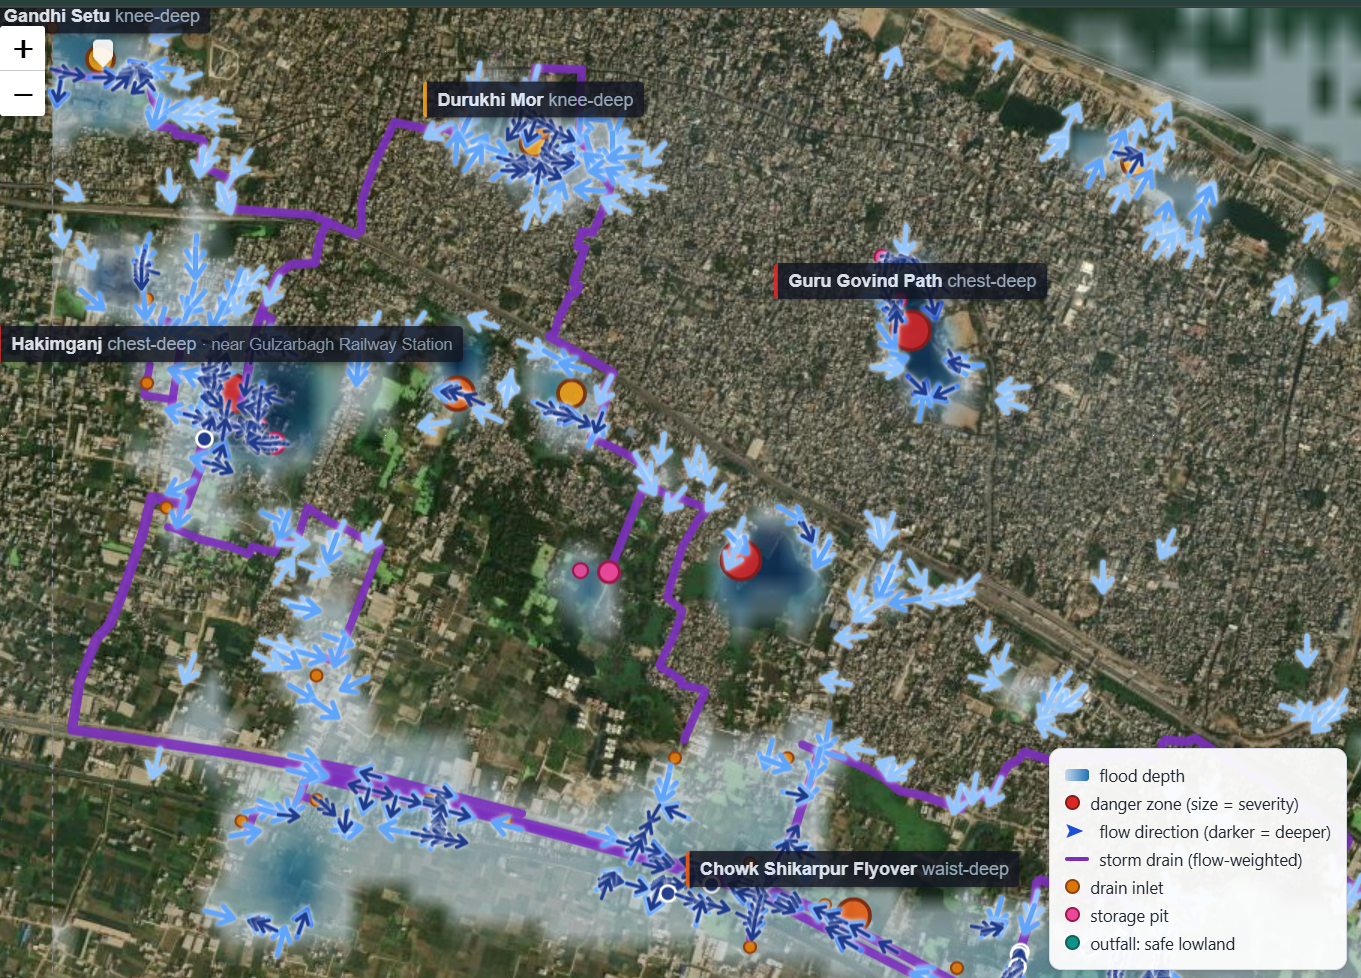
\includegraphics[width=0.99\linewidth]{figures/live_patna_sat.png}
\caption{The designed drain network over satellite imagery for eastern Patna. Purple lines are the
planned trunks, orange circles are inlets, and the arrows are the simulated flow field. The labels
are real road names carrying a predicted depth in words. The network is not drawn by hand. It is
the union of gravity-cheapest exit paths from 40 basin inlets to safe outfalls.}
\label{fig:patnasat}
\end{figure}

\textbf{Results.} Across the eight built areas the spiderweb cuts street flooding by 80.9\,\% in
Patna, 89.4\,\% in Patna-East, 80.3\,\% in Patna-West, 72.6\,\% in Bengaluru, and 63.0, 50.2, 39.2
and 32.5\,\% on the Mumbai South, East, West and North tiles, against 21 to 26\,\% for the sparse
plans. Dose-response over 25 to 200\,mm is monotone.

Density improves the \emph{economics} as well as the effectiveness. Patna costs \rupee850 per cubic
metre removed against \rupee1\,309 for the sparse plan, and Bengaluru costs \rupee1\,121, because
shared trunks spread their length across many basins. The lower Mumbai cuts are informative rather
than disappointing. Those tiles are four times larger, far denser and partly harbour, so a fixed
budget of about 40 inlets covers a smaller share of the flooding.

\subsection{Buildable and phased distributed storage}
The storage planner answers a different question. How many detention tanks, and where, to cut the
flood by a target percentage? Candidate cells are the dynamic local minima of the simulated flood,
ranked by pooled depth. Each site is sized to the water it actually holds, and the cut is
re-measured by simulation rather than assumed.

The important word is buildable. Building footprints and permanent water are excluded from
candidacy, because you cannot dig a tank under an occupied house or in the harbour. Under-street
detention stays allowed, which mirrors how Indian cities actually retrofit. Buildability is not
free on flats. Excluding building-footprint minima removes some of the deepest candidates and the
reachable ladder drops accordingly. We report that rather than quietly siting tanks inside houses.

Each area ships an explicit ranked site list of up to 1\,500 sites with coordinates, per-site
volume and an under-street flag, where 63 to 87\,\% of sites land under streets, together with a
phase ladder costed at indicative rates. Patna reaches a measured 10\,\% cut with 193 sites at
about \rupee165 crore. Mumbai-West needs 493 sites and about \rupee825 crore for the same 10\,\%.
Dense tiles reach 10\,\% and no further, which is an honest ladder rather than an aspirational one.

The planner has never seen a flood report or a news archive. Its top-ranked sites nonetheless land
on each city's chronically flooded places, including Koramangala in Bengaluru and the Mithi at
Kalina in Mumbai-West. Fig.~\ref{fig:mumbai} shows the Mumbai island city network concentrating on
the Parel, Dadar and Byculla belt, which is the Hindmata neighbourhood where the municipal
corporation actually built its underground detention tanks. That coincidence is a qualitative
check. Deep simulated minima on buildable ground fall where flooding actually hurts.

\begin{figure}[!t]
\centering
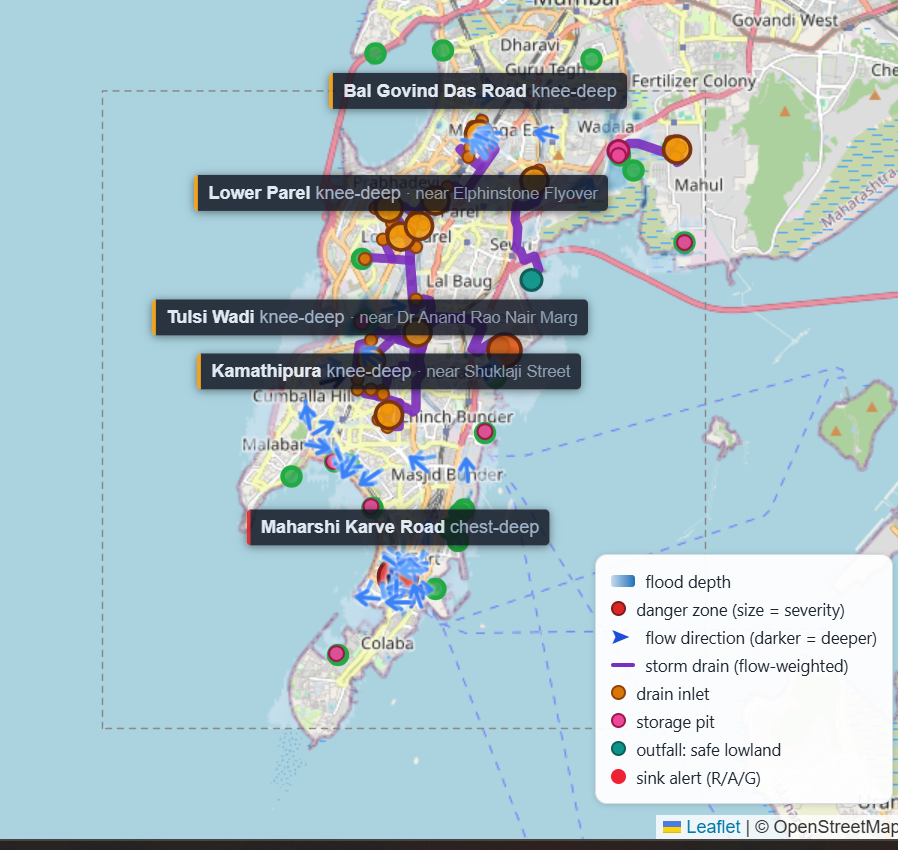
\includegraphics[width=0.99\linewidth]{figures/live_mumbai_city.png}\\[2pt]
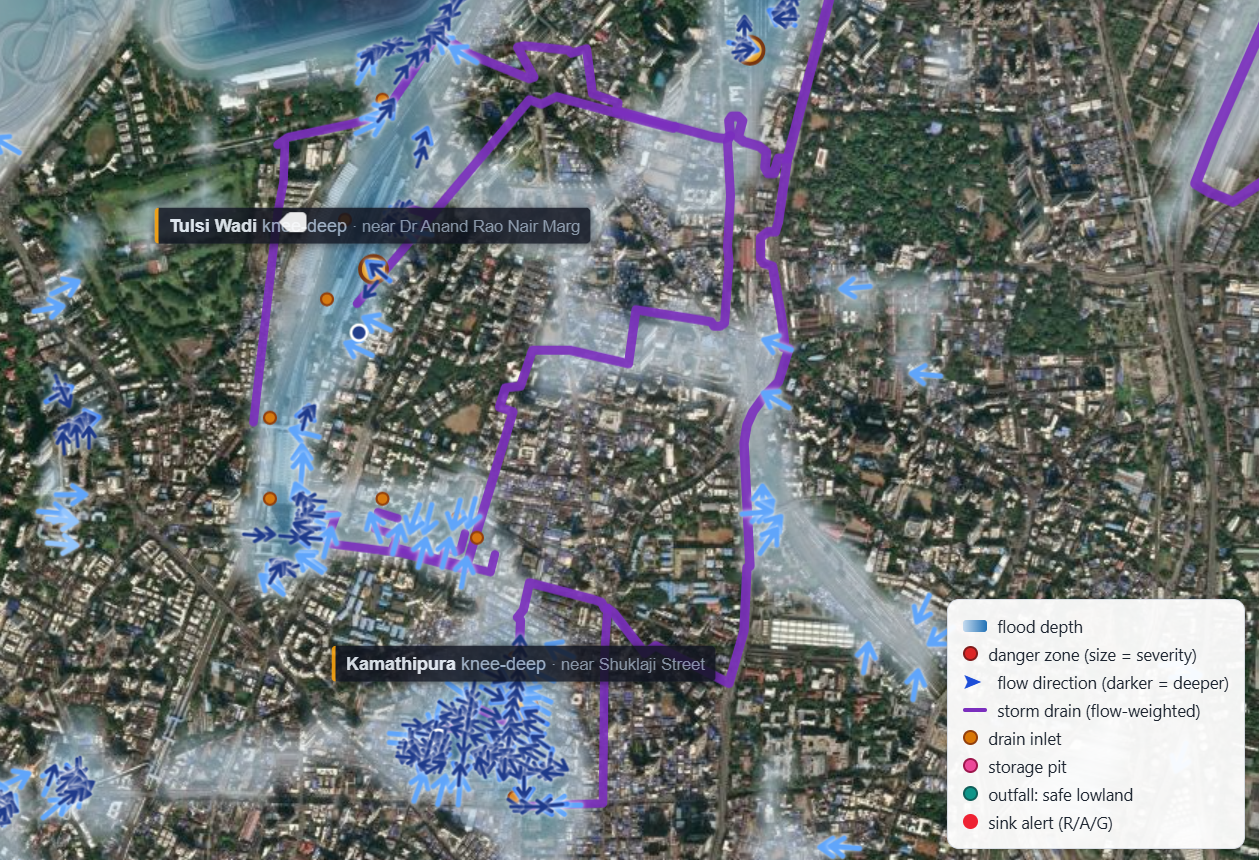
\includegraphics[width=0.99\linewidth]{figures/live_mumbai_sat.png}
\caption{Mumbai island city. \textbf{Top:} the planned network for the whole tile, with labelled
streets at knee and chest depth through Lower Parel, Kamathipura and Tulsi Wadi. Green circles are
safe-lowland outfalls and pink circles are storage pits. \textbf{Bottom:} the same plan over
satellite imagery. The trunks follow the street grid because that is where gravity and buildability
agree.}
\label{fig:mumbai}
\end{figure}

\subsection{Why we trust these decisions given Section~\ref{sec:dem}}
The quantities that drive the plans are the ones the elevation ensemble shows to be robust. Those
are total flooded volume, the existence of a basin, the approximate ordering of depths, and the
downhill topology. They are not the exact street that ponds first. The planner's outputs are also
portfolios, made of many inlets and many small basins, whose value degrades gracefully if any single
pond turns out to be somewhere else. We therefore frame the outputs as relative planning guidance,
meaning which strategy, at what density, and where to start, rather than as certified absolute
depths.

\section{From Flood to Aquifer: Metered Recharge}
\label{sec:recharge}

The water that floods an Indian city in July is water the same region is short of in April. Managed
aquifer recharge is the idea of deliberately putting storm water underground instead of letting it
run off, and it is well studied \cite{mar2026, pavelic2015utfi}. What is usually missing is a
measurement. Most recharge plans assume an infiltration rate and multiply.

We can do better, because we have a physical model that already meters infiltration against a finite
soil capacity, as described in Section~\ref{sec:system}. So we can build recharge structures into the
model, re-simulate the storm, and read off how much water actually went underground rather than
assuming it.

\subsection{Tier A, a state-wide screen}
Choosing where to even build a twin is itself a decision, and doing it by intuition would undo the
point. We screen an entire state first. For each of Karnataka's 27 district units we combine four
free datasets. Central Ground Water Board stage-of-extraction gives the annual ratio of water taken
out to water going in, so above 100\,\% means the aquifer is being mined. A GRACE-assimilated
storage trend gives the direction of change. HydroSHEDS flow accumulation says where runoff
concentrates, because recharge needs water to arrive. SoilGrids conductivity and WorldCover
pervious fraction say whether the ground can take it. The four terms are weighted 0.45 for need,
0.25 for water, 0.15 for soil and 0.15 for land.

The screen ranks Bangalore Rural first at 111\,\% extraction, then Chitradurga at 144\,\%,
Chamarajanagara at 96\,\%, Kolar at 180\,\% and Bangalore Urban at 187\,\%. All are officially
over-exploited or critical.

Two honesty notes travel with this screen. The storage trend input turns out to be effectively
constant across the state, so it contributes nothing to the ranking, and we say so in the artifact
rather than stretching a flat input into apparent signal. And a screen is not a siting. It can say
that a district is depleted \emph{and} has concentrated runoff \emph{and} has pervious ground. It
cannot say build here. Only a re-simulated twin earns a claim in cubic metres.

\subsection{Tier B, twins for six towns, and the measurement}
We then built full 60\,m twins for six Karnataka towns and ran the recharge planner in each, along
with the flood-plain and coastal areas already built. The planner places recharge structures on
pervious ground where water collects, sizes each one, re-simulates, and reports the water that
crossed into the soil column.

\begin{table}[!t]
\centering
\caption{Metered recharge at a 100\,mm storm. Recharge is water that entered the soil column in the
re-simulated model, not an assumed rate. The flood cut column is the measured reduction in street
flooding from the same structures. The plateau towns bank an order of magnitude more of their runoff
than the flood plain and the coast do.}
\label{tab:recharge}
\begin{tabular}{lrrrr}
\toprule
area & sites & recharge (m$^3$) & of runoff & flood cut \\
\midrule
\multicolumn{5}{l}{\emph{Karnataka plateau}}\\
Chikkaballapur   & 4\,323 & 607\,172 & \textbf{16.5\,\%} & 62.7\,\% \\
Kolar            & 4\,875 & 667\,548 & \textbf{14.1\,\%} & 46.9\,\% \\
Doddaballapura   & 4\,122 & 503\,986 & \textbf{10.0\,\%} & 85.4\,\% \\
Chamarajanagara  & 5\,215 & 418\,956 & \textbf{8.1\,\%}  & 88.2\,\% \\
Chitradurga      & 3\,850 & 320\,138 & \textbf{8.0\,\%}  & 49.2\,\% \\
Ramanagara       & 3\,119 & 322\,204 & \textbf{6.3\,\%}  & 76.8\,\% \\
\midrule
\multicolumn{5}{l}{\emph{Flood plain and coast}}\\
Patna-East       & 3\,159 & 102\,013 & 3.3\,\% & 38.4\,\% \\
Patna-West       & 3\,277 & 139\,793 & 2.6\,\% & 22.4\,\% \\
Bengaluru        &    986 &  74\,196 & 1.6\,\% & 4.3\,\% \\
Mumbai-North     & 3\,654 & 114\,711 & 1.1\,\% & 6.2\,\% \\
Patna            & 1\,188 &  32\,714 & 0.7\,\% & 9.1\,\% \\
Mumbai-East      & 2\,693 &  21\,171 & 0.2\,\% & 14.4\,\% \\
Mumbai-West      & 1\,573 &  16\,117 & 0.2\,\% & 7.6\,\% \\
Mumbai-South     &    507 &    $-$534 & 0.0\,\% & 3.7\,\% \\
\bottomrule
\end{tabular}
\end{table}

Table~\ref{tab:recharge} is the result, and the split is the point. The six Karnataka towns send
6.3 to 16.5\,\% of a 100\,mm storm's runoff into the aquifer. The flood plain and the coast manage
0.7 to 3.3\,\%, and Mumbai-South is indistinguishable from zero. That gap is exactly what the
screen predicted and it has a physical reason. On a flood plain the water table is already close to
the surface and the soil column is nearly full, so there is nowhere to put the water. On the
Karnataka plateau the aquifer is mined, hard rock sits under thin soil, and the storage the water
is being invited into is real and empty.

The same structures also cut flooding, by 46.9 to 88.2\,\% in those towns, so this is not a trade
between flood control and water supply. In the places where recharge works, it is the same
intervention.

Fig.~\ref{fig:kolar} shows Kolar, the second-ranked town, with its flood field and the planned
network. Phasing it is costed the same way as storage. Kolar reaches a 10\,\% flood cut with
3\,296 structures holding 6.94 million\,m$^3$, at an indicative \rupee2\,500 per m$^3$ and about
\rupee1\,735 crore.

\begin{figure}[!t]
\centering
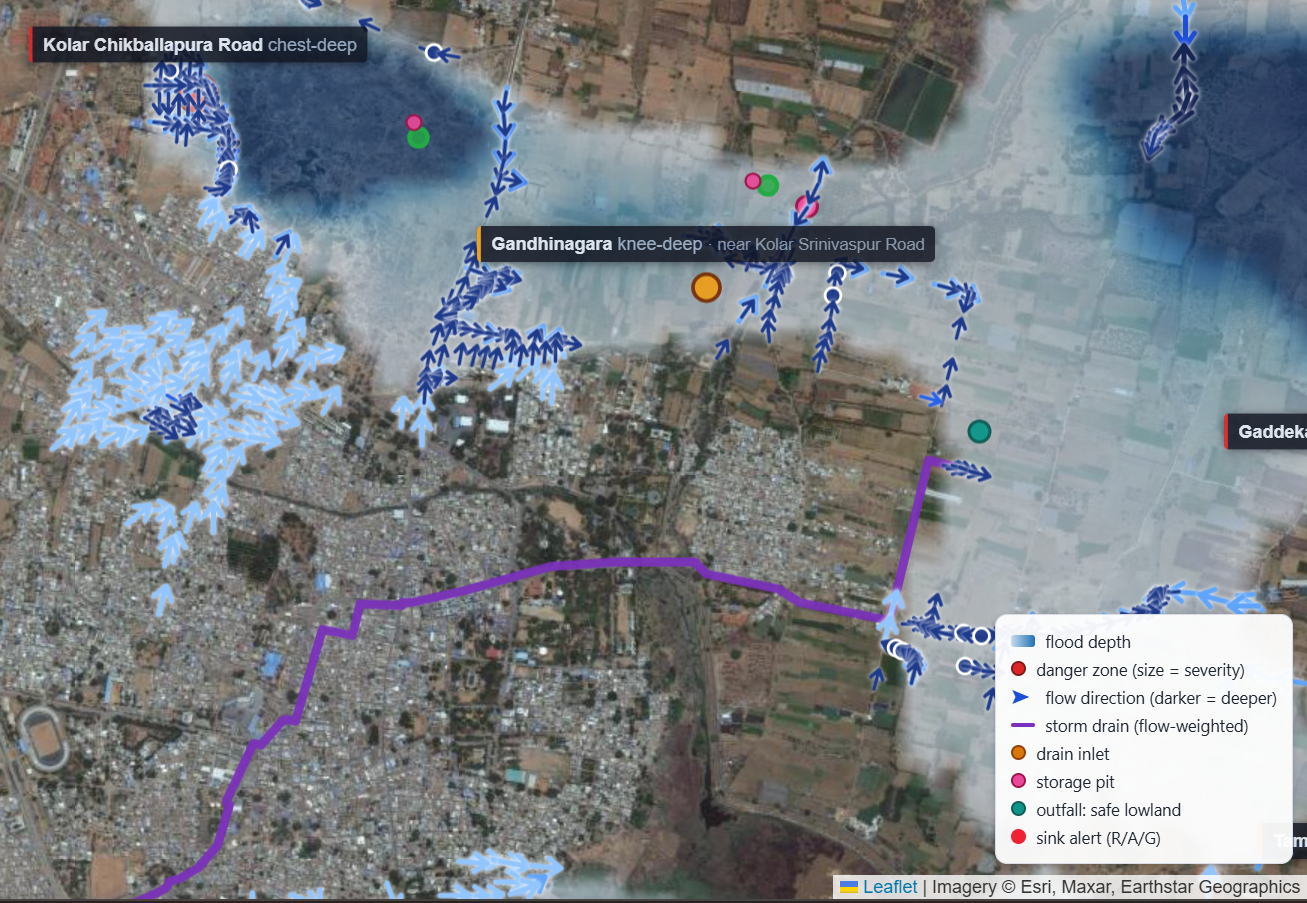
\includegraphics[width=0.99\linewidth]{figures/live_kolar.png}
\caption{Kolar, one of the six Karnataka towns, at a design storm. Kolar district runs at 180\,\%
groundwater extraction, meaning it takes out nearly twice what goes in each year. Blue is predicted
water, arrows are flow, the purple line is the planned trunk to a safe outfall in green, and the
pink circles are storage. Water that currently floods Kolar Chikballapura Road is water the aquifer
under it needs.}
\label{fig:kolar}
\end{figure}

\subsection{What this result does not license}
Two caveats sit on top of these numbers and both are load-bearing.

The recharge \emph{volumes} come from the twin's metered infiltration and depend only on the
physics and the terrain. The site \emph{rankings} additionally use local groundwater level data,
and the well files currently shipped are sample placeholders rather than real measurements, with
the nearest genuine station far outside the area. So the volumes stand and the within-town ordering
of sites should be treated as provisional until Central Ground Water Board station records are
attached. We ship that distinction in the artifact instead of hiding it.

Recharge also has a water quality dimension that a flood model cannot see. Putting urban runoff
underground puts whatever is in that runoff underground too, including sewage and heavy metals.
Parts of Bihar's shallow alluvium carry arsenic, and Karnataka's hard-rock aquifers carry fluoride.
Any real structure needs geotechnical and water-quality screening before construction. This planner
prioritises. It does not certify.

\section{Learned Street-Level Risk, and Routing People Around Water}
\label{sec:gnn}

Both planning surfaces above route on graphs with hand-set costs. We now replace the hand-set cost
with a learned one, and in doing so answer a different question. A planner asks where to build. A
person standing in the rain asks which way to walk.

\subsection{FloodGNN}
FloodGNN is an edge-conditioned message-passing network \cite{gilmer2017} over the OpenStreetMap
street graph, with four rounds of message passing, 96-dimensional states and about 439\,k
parameters. Message passing means each street repeatedly exchanges information with the streets it
connects to, so a street can learn that it is at the bottom of a basin even though nothing in its
own features says so. The network is conditioned on rainfall by FiLM \cite{perez2018film}, which
lets one model cover a continuous range of storm sizes instead of one model per storm.

Node features are deliberately local and standardised per graph. They are elevation anomaly,
pit-ness, grade, flow accumulation, permanent water, radar waterlogging frequency, and building and
road density. Nothing in them identifies the city, which is the property that makes transfer
possible at all.

Supervision is generated by the twin itself. The emulator's depth fields over a 20 to 240\,mm sweep
are sampled at street nodes and edges, and the drain planner's conveyed volume is sampled at three
configurations. That is about nine seconds of label generation per city on a CPU. Wet targets carry
the same twenty-fold loss weight as the emulator, validation holds out \emph{storm sizes} rather
than nodes, and the shipped checkpoint is the best-validation epoch.

\begin{table}[!t]
\centering
\caption{FloodGNN per area. Edge AUC is measured on held-out storm sizes. AUC is the probability
that a randomly chosen flooded street is ranked above a randomly chosen dry one, so 0.5 is chance
and 1.0 is perfect. The last columns compare a full-graph risk query against the raster pipeline it
replaces, on the same hardware.}
\label{tab:gnn}
\begin{tabular}{lccccc}
\toprule
area & nodes & edge AUC & GNN & emulator & speed-up \\
\midrule
Patna       & 37\,017 & \textbf{0.906} & 4.1\,ms & 260.2\,ms & 63$\times$ \\
Patna-East  & 13\,590 & \textbf{0.942} & 3.9\,ms & 110.9\,ms & 28$\times$ \\
Patna-West  & 31\,961 & \textbf{0.890} & 4.1\,ms & 216.0\,ms & 53$\times$ \\
Bengaluru   & 31\,675 & \textbf{0.916} & 5.0\,ms & 238.4\,ms & 48$\times$ \\
\bottomrule
\end{tabular}
\end{table}

\subsection{Risk, and what the message passing buys}
Table~\ref{tab:gnn} gives per-street flood risk at any rainfall in a single forward pass, at 0.89
to 0.94 AUC on held-out storm sizes, in about 4\,ms against 260\,ms for the raster pipeline.

An ablation says the graph structure is earning its place rather than decorating it. Replacing
message passing with a per-node multilayer perceptron that sees the identical features drops Patna
from 0.906 to 0.866, Patna-East from 0.942 to 0.908, Patna-West from 0.890 to 0.879 and Bengaluru
from 0.916 to 0.888. The gain is monotone in the number of rounds, at 0.866 with none, 0.890 with
two and 0.906 with four on Patna. Neighbourhood structure carries signal beyond what purely local
topography explains, which is exactly what a basin is.

We also report what does not work. The flow head recovers the drain planner's trunk ranking only
weakly, with Spearman correlation of 0.14 to 0.24. That is usable for suggesting corridors in the
dashboard, but trunk placement remains the planner's job. The network predicts \emph{wetness} well
and \emph{flow direction} poorly, and we report the number rather than the claim.

\subsection{Zero-shot transfer between cities}
Trained with Bengaluru held out entirely, which makes the training set all flat, FloodGNN ranks
flooded Bengaluru streets at 0.721 AUC without ever seeing the city, against 0.916 when Bengaluru
is in training. The reverse direction is stronger. Held-out Patna scores 0.847 against 0.906,
because a mixed flat and hilly training set already covers Patna's regime.

This is the learned counterpart of Section~\ref{sec:transfer}. Street-level flood knowledge is
substantially city-transferable even where cell-level location is not, and it is hardest going into
a terrain type absent from training, which is the same lesson the coastal experiment taught at the
raster level.

\subsection{Routing}
Given per-street risk, routing is a shortest-path problem with an inflated cost, so that crossing
deep water is expensive but not forbidden. We evaluate on 150 random origin and destination pairs
per area at 140\,mm, judging every route on the true depths so that no method is scored on its own
beliefs. Three routers compete. The flood-ignorant shortest path, FloodGNN, and an oracle that
reads the emulator directly.

\begin{table}[!t]
\centering
\caption{Flood-aware routing, 150 routes per area, all judged on oracle depths. Wet metres is the
flooded street distance an average route crosses. Detour is the extra length against the shortest
path. Avoidance recovered is how much of the oracle's improvement the GNN captures.}
\label{tab:routing}
\begin{tabular}{lcccc}
\toprule
area & shortest & \textbf{GNN} & oracle & recovered \\
\midrule
Patna       & 2\,297\,m & \textbf{1\,570\,m} & 1\,172\,m & \textbf{64.6\,\%} \\
Patna-East  &    585\,m & \textbf{406\,m}    &    369\,m & \textbf{82.9\,\%} \\
Patna-West  & 2\,024\,m & \textbf{1\,727\,m} & 1\,349\,m & \textbf{44.0\,\%} \\
Bengaluru   & 1\,888\,m & \textbf{1\,172\,m} & 1\,333\,m & \textbf{129\,\%} \\
\bottomrule
\end{tabular}
\end{table}

On Patna the learned route crosses 1\,570\,m of flooded street against 2\,297\,m for the
flood-ignorant path and 1\,172\,m for the oracle. That recovers 64.6\,\% of the oracle's
improvement while taking a 21.2\,\% detour against the oracle's 37.1\,\%. In other words it buys
roughly two-thirds of the benefit for a little over half the walking.

\textbf{On Bengaluru the learned router beats the oracle.} It crosses 1\,172\,m against the
oracle's 1\,333\,m. This is not a mistake and it is worth explaining, because it looks like one.
The oracle is greedy on true depth, minimising a risk-inflated cost step by step, and that is not
the same objective as minimising wet metres. The GNN's risk field is smoother, having been produced
by message passing that averages over neighbourhoods, and a smoother field finds a better global
path. An oracle is only optimal for the objective it actually optimises.

\begin{figure}[!t]
\centering
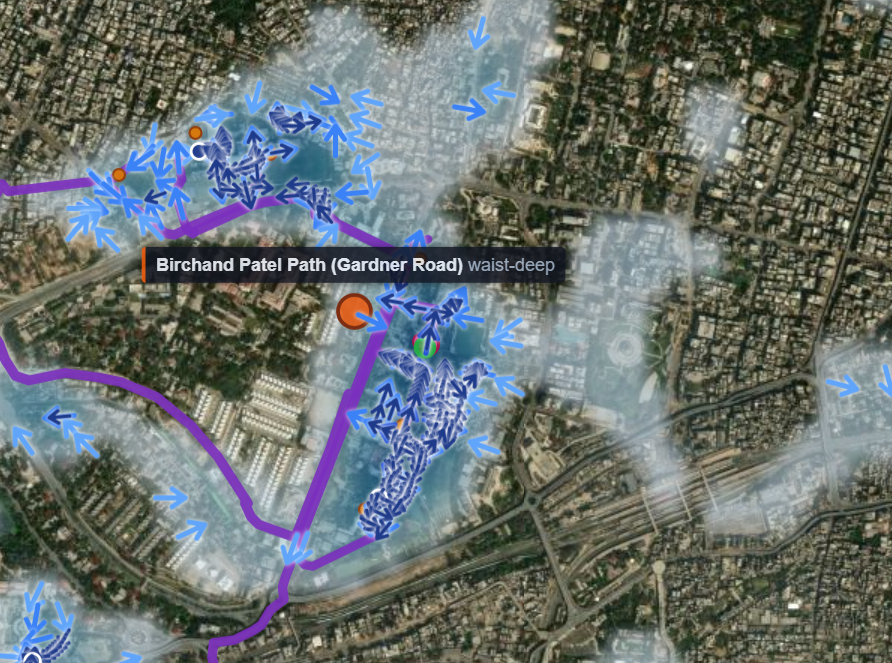
\includegraphics[width=0.99\linewidth]{figures/live_patna_route.png}
\caption{Flood-aware routing in the deployed system. The purple line is the recommended route,
orange circles are street nodes the router refuses to cross, the arrows are the predicted flow
field, and the label names the specific road that is impassable. The full-graph risk query behind
this view takes about 4\,ms, which is why the route updates as the rainfall slider moves.}
\label{fig:route}
\end{figure}

\subsection{Honesty and deployment}
FloodGNN distils the twin, so it inherits the twin's biases. Its claims are amortization, routing
quality \emph{under} the twin's flood fields, and transfer. They are not co-location skill, which
Section~\ref{sec:twin} shows the twin itself largely lacks and which a model learned directly from
terrain does have. Supervising directly on radar-observed street water is the natural next step and
we have not done it.

The 1.8\,MB checkpoint ships inside the dashboard image. The routing endpoint answers from the GNN
where a checkpoint exists and from the raster emulator otherwise, and it reports which backend
answered.

\section{The Deployed System and Its Learning Gate}
\label{sec:live}

Everything above is computed from satellites and simulation. The people being flooded know things
neither can see. The deployed system closes that loop under strict honesty constraints, and we
report the loop's status accurately, which is that its machinery works and its evidence does not
yet exist.

\subsection{Citizen reports as data}
Dashboard users drop a pin with a water level they can actually judge, being ankle, knee, waist or
chest, mapped to depth bands with explicit tolerances of $\pm$0.15 to 0.35\,m, plus an optional
note. This is why the labels in Fig.~\ref{fig:teaser} are words rather than numbers. A person can
confirm or contradict ``knee-deep''. Nobody can confirm 0.47\,m.

Reports are validated against the area's model window and rate-limited by salted address hash, with
five per hour, a per-cell cool-down, a global daily cap and a honeypot field for bots. They are held
in memory for the live map and mirrored by a background scheduler to a public dataset repository,
which doubles as durable storage across free-tier restarts. No personal data is served, and the
hashes never leave the backend.

\subsection{From reports to supervision}
A report is only a label together with the storm that caused it. The nightly job groups reports by
calendar day in local time, tags each day with the rainfall that actually fell, and drops dry days
below 5\,mm. A knee-deep report without rain is far more likely to be mischief or a burst pipe than
a storm signal. Same-cell same-day reports collapse to their median, so one street corner cannot
dominate.

\subsection{The reward gate}
Citizen reports carry no dry labels, so a model that predicts deep water everywhere would score
perfectly on wet points. That is the same failure mode as the emulator's sparse targets, now in the
field, and it is why the loop needs a gate rather than a learning rate.

A candidate emulator is fine-tuned with a band-tolerant loss on report points, meaning zero gradient
inside the reported band, anchored by a simulation replay buffer in every batch. It ships only if
all four of the following hold. There are at least 15 held-out points from at least two distinct
storm days, held out \emph{by day} because points within a day are correlated. Held-out point error
improves by at least 5\,\%. Replay error degrades by at most 10\,\%, which is the all-wet guard. And
it wins at least 70\,\% of bootstrap resamples of the held-out errors.

Every decision, accepted or held, with all four numbers, is appended to a public learning log
surfaced on the dashboard, so the loop is auditable by the people whose reports feed it.

\textbf{Status, stated plainly.} The loop is deployed and the gate is tested offline. The refresh
half, which pulls weather and recomputes outlooks, runs end to end. The learning half has never
fired, because the reports dataset is empty. Running it nightly today would produce a log of nights
with zero model updates, which is the correct behaviour and not a result. We therefore claim a
mechanism and an audit trail here, and no learning outcome. The first accepted or correctly refused
field update remains the most interesting experiment we have not been able to run.

\subsection{Live context layers}
The same discipline applies to the ambient layers. Live forecast alerts recompute the outlook
read-only and never mutate committed artifacts. Advisories are generated in English, Hindi and
Marathi from only the system's own numbers, with a deterministic template fallback so the panel
works with no language model at all. A Black Marble night lights overlay \cite{roman2018} marks
built-up cells whose latest good-quality night radiance dropped more than 50\,\% below their 90-day
median, which is a proxy for a power outage.

One trap there is worth recording for anyone building the same layer. During monsoon cloud cover a
fully quality-masked composite downloads as \emph{zero radiance}, which reads naively as a city-wide
blackout. Missing data must be treated as unknown and not as dark.

\section{Limitations}
\label{sec:limits}

\textbf{Resolution.} The hydraulics run at 60\,m, which is coarser than the streets they describe.
Carved drains are full 60\,m cells, so absolute excavation volumes are resolution artifacts even
though the per-metre drain costing is realistic. Section~\ref{sec:twin} measures the consequence
directly. Depth is diluted by a factor of 4.45, implying a real ponding footprint near 28.5\,m
across. A finer grid is the single clearest next step, and it has a quantitative target.

\textbf{Depths are uncalibrated,} and Section~\ref{sec:dem} shows why per-class physics calibration
cannot fix location inside the solver, even though a learned model on the same rasters can.

\textbf{The evidence base is uneven.} The like-for-like comparison of Table~\ref{tab:baselines}
rests on 18 storms across two areas, because those are the only areas with a twin baseline to
compare against. Everything after it rests on 15 areas and 150 scenes. We consider re-measuring the
like-for-like table across all 15 areas the most valuable single experiment we have not run.

\textbf{Mumbai has regime-specific caveats.} The tiles are independent closed-boundary models, so
flow across the seams is not simulated. Tidal and storm-surge coupling, often the binding
constraint for Mumbai outfalls, is absent, and rain falling on harbour cells ponds harmlessly inside
the model instead of exchanging with the sea. Mumbai-Harbour is excluded from headline validation
because its observed water is almost entirely persistent, with a storm increment of exactly zero on
8 of its 11 dates, so it measures a different hazard than urban rain flooding. A calendar-derived
tide phase does not explain it, with a permutation test at $p = 0.47$, and a real tide gauge remains
untested.

\textbf{The coastal result rests on two cities.} One coastal sibling raises held-out Mumbai by
84\,\% without closing the gap to inland performance, and Chennai's own figure rests on ten scenes.
Whether coastal skill keeps climbing with a third coast or plateaus is unresolved, and it is a
cheap experiment.

\textbf{Recharge site rankings use placeholder well data,} as stated in Section~\ref{sec:recharge},
while the recharge volumes come from the twin's metered infiltration and do not depend on it.

\textbf{Costs are indicative.} Phase costs use a single civil-works rate. Land, utilities and
operations are out of scope, so the ladders rank strategies rather than price projects.

\textbf{The learning loop is unexercised.} Its gate is deployed and tested offline, and no field
report has ever reached it.

\textbf{Routing is evaluated on synthetic trips.} The 150 origin and destination pairs per area are
random, not observed journeys, and the oracle they are measured against is greedy rather than
optimal.

\textbf{What we would do next.} A finer national elevation model, assimilating mapped drain networks
where cities have them, sub-grid street conveyance, supervising FloodGNN directly on radar-observed
street water to remove the ``distils the twin'' caveat, tidal boundaries for coastal tiles, a third
coastal city, and validating intervention \emph{deltas} rather than state against before and after
radar where a city has actually built drainage.

\section{Conclusion}

We built a working urban flood twin for 16 Indian city areas out of free satellite data, on free
computing, and put it on the public internet. That part is engineering. The part we think matters
more is what happened when we measured it properly.

A flood overlap score on this task is uninterpretable on its own. A baseline with no physics, no
rainfall and one fixed parameter scores 0.29 to 0.67 across 15 areas, beating every physics-model
score we can find published, and beating the agreement between two radar passes of the same city in
all fifteen. Any CSI in this literature, ours included, should be read next to those numbers or not
read at all.

Once that scale is fixed, the rest of the results change shape. Our physics twin scores 0.054 and a
learned model on the identical rasters scores 0.288, which refutes our own earlier claim that
terrain fundamentally lacks the information. But that same learned model ties the parameter-free
baseline exactly, so its value is not accuracy. Its value is that it runs on cities with no radar
history at all, and held out one whole region at a time that is worth 0.147, rising to 0.175 with a
threshold correction that costs nothing and never looks at a test label. The one place it nearly
fails is a coast it has not seen, and we showed that is a coverage problem rather than a hard
limit, because adding a single coastal city lifted held-out coastal skill by 84\,\%.

Three things that ought to have helped did not. Model size across a 35-fold range did nothing.
Grid resolution from 60 to 30\,m did nothing. Rainfall from free reanalysis did nothing at best and
actively hurt at worst, shown four independent ways with two alternative explanations refuted.

Meanwhile planning works despite the location uncertainty, because we measure every intervention by
re-simulation instead of assuming it. A dense street-routed drain network cuts simulated street
flooding by 80.9\,\% in Patna and costs less per cubic metre than the sparse alternative. A metered
recharge planner banks 6.3 to 16.5\,\% of a storm's runoff in six depleted Karnataka towns against
0.7 to 3.3\,\% on the flood plain, and cuts flooding at the same time. An inferred drainage field
puts a falsifiable ceiling on Mumbai's whole-city drainage near 5.4 million cubic metres per storm,
which sits on the correct side of the 4.7 million cubic metres per day the city measured itself
pumping. And a graph network over the streets makes all of it fast enough to route a person around
the water in four milliseconds.

We have reported the failures beside the successes throughout, including three corrections against
our own published claims, a negative result against 83 crowdsourced depth measurements, a drainage
inversion that improved the quantity it was trained on and did nothing for the one that matters,
and a learning loop whose gate has never fired because nobody has filed a report yet. We would
rather the record be useful than flattering.

\section*{Reproducibility}
Code, all per-area artifact bundles including the Sentinel-1 water masks for the 15 areas that have
them, road graphs, replay buffers and ranked site lists, together with 253 offline tests and
step-by-step runbooks, are public at
\url{https://github.com/Maverick-Ansh/project-varuna}. The live dashboard is at
\url{https://project-varuna-iota.vercel.app} and its API at
\url{https://anshvivek-varuna-floodtwin.hf.space}.

A new city builds with one script on a free GPU and serves from the committed bundle. Every headline
number in this paper is regenerable from a committed artifact. The learned-baseline dataset is
rebuilt by three builders, each with a verify mode that reports agreement with the committed copy
rather than asserting it. The headline is unchanged on a fully rebuilt dataset, at
$0.288 \pm 0.008$ against $0.288 \pm 0.007$. The trivial-baseline builder reproduces all previously
published values before extending them, which is how the fifteenth area was added to
Table~\ref{tab:trivial} without disturbing the other fourteen. Sentinel-1 masks for a new area are
fetched by a script that needs one interactive Earth Engine login and ranks candidate dates by
antecedent rainfall, so scenes are chosen for having weather in them rather than by hand.

\section*{Acknowledgment}
This work uses FABDEM, ESA WorldCover, JRC Global Surface Water, Copernicus Sentinel-1,
OpenStreetMap, Open-Meteo, NASA Black Marble, SoilGrids, HydroSHEDS and Central Ground Water Board
data, all of which are free to use. The crowdsourced depth observations come from the public
mumbaiflood.in service. The system runs on free tiers provided by Google Colab, Kaggle, Hugging Face
and Vercel. None of this work would be possible if those datasets and services were not open.



\bibliographystyle{IEEEtran}
\bibliography{varuna-ieee}

\end{document}
